\documentclass[12pt, a4paper, oneside, UTF8]{ctexart}
\pagestyle{plain}	% 去除页眉
\usepackage{amsmath, amssymb, graphicx}
%生成pdf书签(中括号内代表给标签加编号)
\usepackage[bookmarksnumbered=true]{hyperref}
%三横线表格的宏包
\usepackage{booktabs}
%避免图片的浮动超过Section部分
\usepackage[section]{placeins}
% 加载 enumitem 宏包以自定义 enumerate 环境
\usepackage{enumitem} 
% 用于并排显示子图
\usepackage{subcaption} 

\usepackage{natbib}

\bibliographystyle{unsrt} % 选择合适的引用格式
% 预先指定图片的搜索路径
\graphicspath{{figure/}}


\title{初识\LaTeX}
\author{匿名}
\date{\today}

%以上部分为导言区
\begin{document}

%封面
\begin{titlepage}
    \centering
    \vspace*{1cm}
    
\includegraphics[width=0.25\textwidth]{logo.png} % 插入校徽
    \vspace{1cm}

    
\includegraphics[width=0.5\textwidth]{name.png} % 插入校名
    \vspace{1cm}

    \huge\textbf{作业论文模板}
    \vspace{1.5cm}

    \Large
    \begin{tabular}{rl}
        %通过underline+makebox来设置下划线长度               
        %若需要加空格显示,使用\hspace{length}          
        %对于汉字使用\hskiplength更合理
        % \large 学生姓名: & \large \underline{\makebox[8em][l]{小明\hskip1em小刚}} \\
        \large 学生姓名: & \large 小明 \\
        \large 学生学号: & \large 2000123456 \\                            
        \large 学科院系: & \large 数学科学学院 \\
        \large 学科专业: & \large 统计数学 \\
        \large 指导教师: & \large 小明 \\
    \end{tabular}
    \vfill

    \large{\today}
\end{titlepage}

\section*{摘要} % 使用 * 来避免在目录中显示摘要
\addcontentsline{toc}{section}{摘要} % 将摘要添加到目录中
用粗糙但高效的启发式规则来豁免那些不太可能是完全加密的流量,然后它阻止其余未被豁免的流量。
这些启发式规则基于常见协议的指纹、1比特的占比以及可打印的ASCII字符的数量、比例和位置。\\ \\
\noindent \textbf{关键词:} 加密协议,流量分析

%正文部分前设置罗马数字
\pagenumbering{Roman}
\newpage
\tableofcontents
\newpage
%正文部分重新设置为阿拉伯数字
\pagenumbering{arabic}

\section{插入数学公式}
此文章是用来练习$LaTeX$的一些基本使用方法。测试参考文献标注,请注意bib文件内的参考文献至少有一个被引用才可以,
先XeLaTeX编译主文件,再使用BibTeX编译一次,然后再使用XeLaTeX编译两次,一共四次\citep{munns2002comparative}
\subsection{数学模式}
在行文中使用\$ ... \$ 可以插入行内公式。如$E=mc^2$.\\
在行文中使用$\backslash$begin\{equation \} ... $\backslash$end\{equation\} 可以插入行间公式。如:
\begin{equation}
E=mc^2.
\end{equation}
或者也可以写成equation*,这样就不会有编号。或者也可以使用$\backslash$[ 数学公式 $\backslash$],
这样也可以表示行间公式。\\在数学模式当中,上标为\^下标为\_并且只作用于之后的一个字符,如需要多个字符,请使用花括号括起来。
对于分式,如果要强制行内模式的分式显示为行间模式的大小,可以使用 $\backslash$dfrac, 
比如:$ \dfrac{1}{2} $
反之可以使用 $\backslash$tfrac
比如:$ \tfrac{1}{2} $,这个大小是与行间强制使用一样的
\subsection{运算符}
连加、连乘、极限、积分等大型运算符分别用$\backslash$sum, $\backslash$prod, $\backslash$lim, $\backslash$int
他们的上下标在行内公式中被压缩,以适应行高。我们可以用 $\backslash$limits 和 $\backslash$nolimits
%\quad means space
来强制显式地指定是否压缩这些上下标。例如:$ \sum_{i=1}^n i\quad \prod_{i=1}^n $
$ \sum\limits _{i=1}^n i\quad \prod\limits _{i=1}^n $
\[ \lim_{x\to0}x^2 \quad \int_a^b x^2 \mathrm{d}{x} \]
\[ \lim\nolimits _{x\to0}x^2\quad \int\nolimits_a^b x^2 \mathrm{d}{x} \]
\subsection{定界符}
在数学模式当中,可以使用大括号、中括号、小括号、单竖线、双竖线、单横线、双横线来表示定界符。
对于竖线$\vert$我们推荐使用$\backslash$vert来表示,而不是$\backslash \vert$,
把v改为大写V则表示双竖线
\subsection{省略号}
省略号用 $\backslash$dots, $\backslash$cdots, $\backslash$vdots, $\backslash$ddots 
等命令表示。$\backslash$dots 和 $\backslash$cdots 的纵向位置不同,前者一般用于有下标的序列。
\[ x_1,x_2,\dots ,x_n\quad 1,2,\cdots ,n\quad
\vdots\quad \ddots \]
\subsection{矩阵}
amsmath 的 pmatrix, bmatrix, Bmatrix, vmatrix, Vmatrix 
等环境可以在矩阵两边加上各种分隔符。
\begin{equation*}
\begin{pmatrix} a&b\\c&d \end{pmatrix} \quad
\begin{bmatrix} a&b\\c&d \end{bmatrix} \quad
\begin{Bmatrix} a&b\\c&d \end{Bmatrix} \quad
\begin{vmatrix} a&b\\c&d \end{vmatrix} \quad
\begin{Vmatrix} a&b\\c&d \end{Vmatrix}
\end{equation*}
当然也可以使用smallmatrix环境,可生成行内公式的小矩阵
$ ( \begin{smallmatrix} a&b\\c&d \end{smallmatrix} ) $
\subsection{长公式}
\subsubsection{不对齐}
无须对齐的长公式可以使用 multline 环境
\begin{multline*}
    x = a+b+c+{} \\
    d+e+f+g
\end{multline*}
\subsubsection{对齐}
需要对齐的公式,可以使用 aligned \textit{次环境}来实现,
它必须包含在数学环境之内,如果使用align则不必。插入\&表示我们希望对齐的位置,
而使用\{\}表示一个空白
\begin{equation*} 
    \begin{aligned}
        x ={}&a+b+c+ \\
             &d+e+f+g
    \end{aligned}
\end{equation*}
\subsection{公式组}
无需对齐的公式组可以使用 gather 环境,需要对齐的公式组可以使用 align 环境。
他们都带有编号,如果不需要编号可以使用带星花的版本。
\begin{gather}
    a = b+c+d \\
    x = y+z
\end{gather}
\begin{align*}
    a &= b+c+d \\
    x &= y+z
\end{align*}
\subsection{分段函数}
分段函数可以用cases\textit{次环境}来实现,它必须包含在数学环境之内。
\begin{equation*}
    y=
    \begin{cases}
        -\sin{x},\quad x \leqslant 0 \\
        x,\quad x>0
    \end{cases} 
\end{equation*}
\section{插入图片和表格}
\subsection{插入图片}
在 LaTeX 中插入图片,有很多种方式。最好用的应当属利用graphicx宏包提供的
$\backslash$includegraphics命令。比如在 TeX 源文件同目录下,有名为 a.jpg 的图片,
可以用这样的方式将它插入到输出文档中:
当然也可以在导言部分使用$\backslash$graphicspath\{路径\}来制定图片的搜索路径.
图片可能很大,超过了输出文件的纸张大小,或者干脆就是你自己觉得输出的效果不爽。
这时候可以用 $\backslash$includegraphics 控制序列的可选参数来控制。
比如$\backslash$includegraphics [ width = .8$\backslash$ textwidth ] \{a.jpg\}。
这样图片的宽度会被缩放至页面宽度的百分之八十,图片的总高度会按比例缩放。
其他的功能可以查看该包的文档\\
\subsection{插入表格}
tabular环境提供了最简单的表格功能。它用 $\backslash$hline 命令表示横线,
在列格式中用 | 表示竖线;用 \& 来分列,
用 $\backslash$$\backslash$ 来换行;
每列可以采用居左、居中、居右等横向对齐方式,分别用 l、c、r 来表示。\\
\begin{equation*}
    \begin{tabular}{|l|c|r|}
        \hline
       操作系统& 发行版& 编辑器\\
        \hline
       Windows & MikTeX & TexMakerX \\
        \hline
       Unix/Linux & teTeX & Kile \\
        \hline
       Mac OS & MacTeX & TeXShop \\
        \hline
       通用& TeX Live & TeXworks \\
        \hline
       \end{tabular}
\end{equation*}
有时候我们需要列出一些总结,可以使用itemize环境与$\backslash$item。而item后面可以跟一个方括号,
中括号内的东西就替换掉默认的黑点,根据需求添加序号,比如下面这个例子
\begin{itemize}
  \item 第一条        
  \item[(2)] 第二条      
\end{itemize}
或者使用下面的enumerate环境紧接方括号内label=$($ $\backslash$arabic*$)$配上自动标号
\begin{enumerate}[label=(\arabic*)]
  \item 自动标号       
\end{enumerate}
除此之外,可以使用 booktabs 宏包中的
$\backslash$toprule、$\backslash$midrule和$\backslash$bottomrule命令。
这些命令提供了更好的表格线样式,并且专门用于创建三横线表格。
\begin{equation*}
    \begin{tabular}{ccccc}
        \toprule
        姓名 & 数学 & 语文 & 英语 & 总分 \\
        \midrule
        张三 & 85 & 90 & 75 & 250 \\
        李四 & 95 & 85 & 80 & 260 \\
        王五 & 80 & 85 & 85 & 250 \\
        \bottomrule
    \end{tabular}
\end{equation*}
当然我们还可以使用插入图片的方式来进行表格的进一步控制,比如在下方添加表的名字,
可以使$\backslash$caption*\{\}的方式从而取消图片的标序,
两个表之间可以手动使用$\backslash$vspace\{2cm\}指定间隔,具体可以查看源代码
\vspace{2cm}
\begin{table}[htbp]
    \centering
    \begin{tabular}{ccccc}
        \toprule
        姓名 & 数学 & 语文 & 英语 & 总分 \\
        \midrule
        张三 & 85 & 90 & 75 & 250 \\
        李四 & 95 & 85 & 80 & 260 \\
        王五 & 80 & 85 & 85 & 250 \\
        \bottomrule
    \end{tabular}
    % 使用*从而取消图片的标序
    \caption*{成绩表}
    \label{tab:grade}
\end{table}

% 或者使用下面的enumerate环境的方法自动标号
% \begin{enumerate}[label=(\arabic*)]
%   \item         
% \end{enumerate}
\subsection{浮动体}
插图和表格通常需要占据大块空间,所以在文字处理软件中我们经常需要调整他们的位置。
figure 和 table 环境可以自动完成这样的任务;
这种自动调整位置的环境称作浮动体(float) 。我们以 figure 为例。
\begin{figure}[htbp]
    \centering
    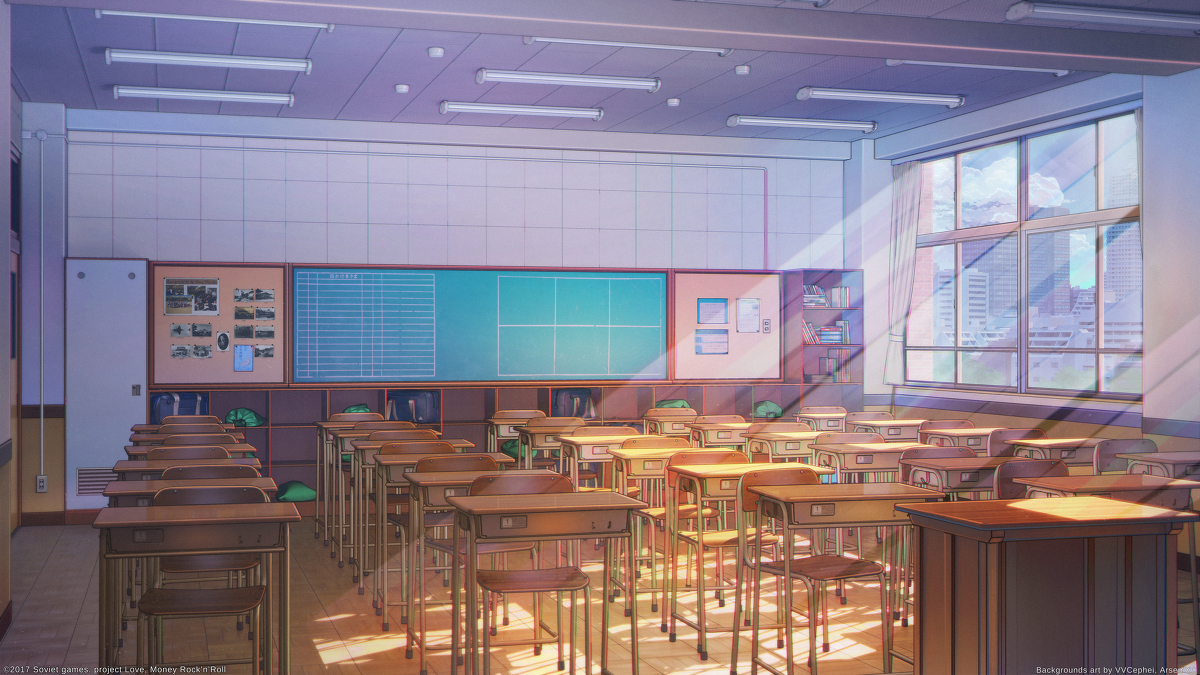
\includegraphics[width = .8\textwidth]{classroom.png}
    \caption{有图有真相}
    \label{fig:myphoto}
\end{figure}
htbp 选项用来指定插图的理想位置,
这几个字母分别代表 here, top, bottom, float page,
也就是就这里、页顶、页尾、浮动页(专门放浮动体的单独页面或分栏)。
$\backslash$centering 用来使插图居中;
$\backslash$caption 命令设置插图标题,
LaTeX 会自动给浮动体的标题加上编号。注意$\backslash$label 应该放在标题命令之后。
但是实际上浮动图片的问题并非想象中的简单,这里碍于时间限制暂时写到这里。
补充一点,如果想让两个图片同行显示可以使用$\backslash$subfigure,效果如下
\begin{figure}[htbp]
    \centering
    \begin{subfigure}[b]{0.45\textwidth}
        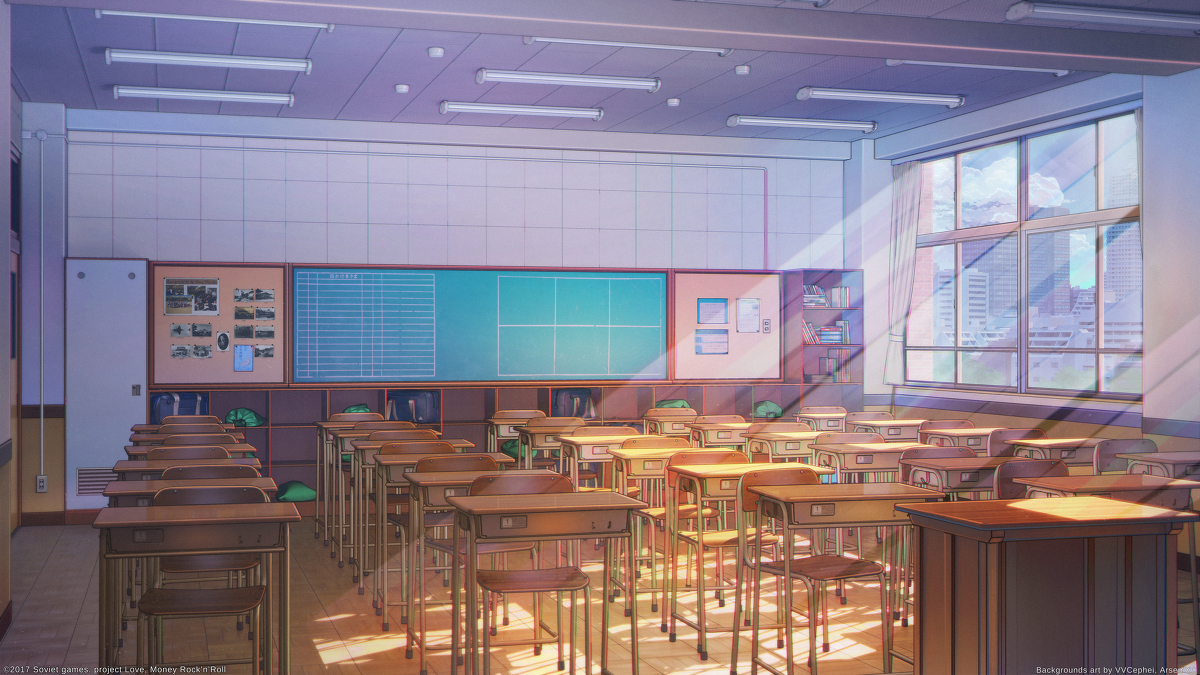
\includegraphics[width=\textwidth]{classroom.png}
        % \caption{}
        \label{fig:image1}
    \end{subfigure}
    \hfill
    \begin{subfigure}[b]{0.45\textwidth}
        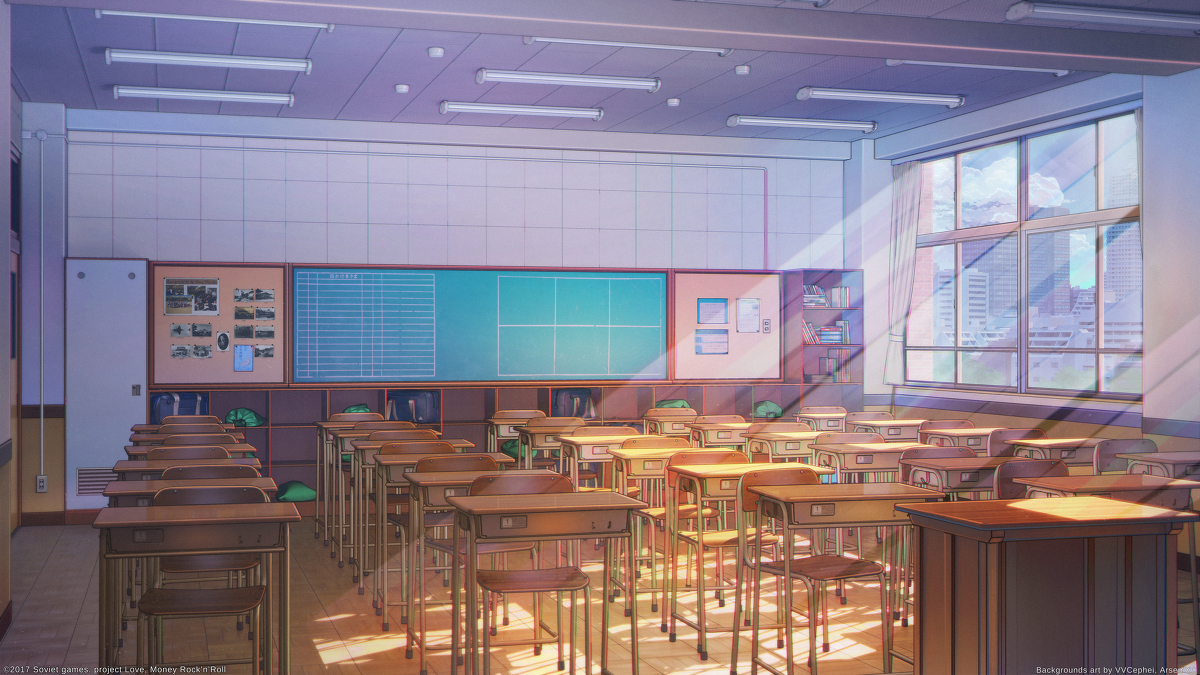
\includegraphics[width=\textwidth]{classroom.png}
        % \caption{}
        \label{fig:image2}
    \end{subfigure}
    \caption{有图有真相2}
    \label{fig:twosubfigs004}
\end{figure}
\section{版面设置}
\subsection{行间距}
\noindent 可以使用$\backslash$noindent指定第一行不缩进。
我们可以通过 setspace 宏包提供的命令来调整行间距。
比如在导言区添加
$\backslash$usepackage\{setspace\}
$\backslash$onehalfspacing,可以将行距设置为字号的 1.5 倍:
请注意用词的差别:行距是字号的 1.5 倍;1.5 倍行距。
事实上,这不是设置 1.5 倍行距的正确方法。
\subsection{段间距}
我们可以通过修改长度 $\backslash$parskip 的值来调整段间距。例如在导言区添加
$\backslash$addtolength\{$\backslash$parskip\}\{.4em\}
则可以在原有的基础上,增加段间距 0.4em。如果需要减小段间距,只需将该数值改为负值即可。
\subsection{字体}
在数学模式中,可以使用$\backslash$textit\{\}, $\backslash$textbf\{\}, 
$\backslash$textsf\{\}, $\backslash$texttt\{\}来表示字体。
%参考文献部分
\newpage
\addcontentsline{toc}{section}{参考文献}
% .bib 文件名(不带扩展名
\bibliography{user}
\end{document}